\documentclass{article}
\usepackage[utf8]{inputenc}
\usepackage[T1]{fontenc}
\usepackage{amsmath, amssymb}
\usepackage{xcolor}
\usepackage{array}
\usepackage{graphicx}
\usepackage{lipsum}
\usepackage{cancel}
\usepackage{polynom}
\usepackage{enumitem}
\usepackage{framed}
\usepackage{hyperref}
\usepackage[most]{tcolorbox}
\usepackage{pgfplots}

% Define colors
\definecolor{examplecolor}{RGB}{92, 184, 92}
\definecolor{lessoncolor}{RGB}{74, 144, 226}
\definecolor{notecolor}{RGB}{255, 179, 102}
\definecolor{solutioncolor}{RGB}{74, 144, 226}

% Define new environment for solutions
\newenvironment{solution}{\color{solutioncolor}}{}
% for small text
\newcommand{\smalltext}[1]{\text{\footnotesize #1}}

\title{Advanced Functions Exam - Part B}
\author{Kensukeken}
\date{May 23rd, 2024}

\begin{document}
\maketitle

\subsection*{Part B: Long Answer}
1. Solve $(\theta \in [0, 2\pi])$
\begin{enumerate}
    \item[a)] $2x^4+4x+4=x^3+9x^2$
    \begin{solution}
        \begin{align*}
            2x^4 + 4x + 4 &= x^3 + 9x^2 \quad \text{(Rearrange all terms to one side)} \\
            2x^4 - x^3 + 9x^2 + 4x + 4 &= 0 \quad \text{(Form polynomial equation)} \\
        \end{align*}
    \end{solution}
    
    \item[b)] $x^4 + x^3 + 3x + 7 > 5x^2 + 7$
    \begin{solution}
        \begin{align*}
            x^4 + x^3 + 3x + 7 &> 5x^2 + 7 \quad \text{(Rearrange all terms to one side)} \\
            x^4 + x^3 - 5x^2 + 3x &> 0 \\
            x(x^3 + x^2 - 5x + 3) &= 0 \quad \text{(Factor out } x \text{)} \\
            x &= 0 \quad \text{(One solution)} \\
\end{align*}
    \end{solution}
    
    \item[c)] $\frac{x^2}{2x^2-5x+3} + \frac{2x}{4x^2-9} = \frac{5}{4x^3 - 4x^2 - 9x + 9}$
    \begin{solution}
       \begin{align*}
\frac{x^2}{2x^2-5x+3} + \frac{2x}{4x^2-9} &= \frac{5}{4x^3 - 4x^2 - 9x + 9} \\
2x^2 - 5x + 3 &= (2x - 3)(x - 1) \\
4x^2 - 9 &= (2x - 3)(2x + 3) \\
\frac{x^2}{(2x - 3)(x - 1)} + \frac{2x}{(2x - 3)(2x + 3)} &= \frac{5}{4x^3 - 4x^2 - 9x + 9} \\
\frac{x^2(2x + 3)}{(2x - 3)(x - 1)(2x + 3)} + \frac{2x(x - 1)}{(2x - 3)(x - 1)(2x + 3)} &= \frac{5}{4x^3 - 4x^2 - 9x + 9} \\
\frac{2x^3 + 3x^2 + 2x^2 - 2x}{(2x - 3)(x - 1)(2x + 3)} &= \frac{5}{4x^3 - 4x^2 - 9x + 9} \\
\frac{2x^3 + 5x^2 - 2x}{(2x - 3)(x - 1)(2x + 3)} &= \frac{5}{4x^3 - 4x^2 - 9x + 9} \\
\frac{2x^3 + 5x^2 - 2x}{(2x - 3)(x - 1)(2x + 3)} &= \frac{5}{(2x - 1)(x - 3)}
\end{align*}

    \end{solution}
    
    \item[d)] $\frac{-4x+1}{x^2-4} < \frac{2x+1}{x+2}$
    \begin{solution}
        \begin{align*}
            \frac{-4x + 1}{(x - 2)(x + 2)} &< \frac{2x + 1}{x + 2} \\
            \frac{-4x + 1 - (2x + 1)(x - 2)}{(x - 2)(x + 2)} &< 0 \\
            \frac{-4x + 1 - 2x^2 + 4x - 2x + 2}{(x - 2)(x + 2)} &< 0 \\
            \frac{-2x^2 + 3}{(x - 2)(x + 2)} &< 0 \\
            x &= \pm 2, \sqrt{\frac{3}{2}} \\
            \text{Test intervals:} & x \in (-\infty, -2) \cup (2, \sqrt{\frac{3}{2}})
        \end{align*}
    \end{solution}
    
    \item[e)] $8.72(0.93)^{x+3} + 17 = 22$
    \begin{solution}
        \begin{align*}
            8.72(0.93)^{x+3} &= 5 \quad \text{(Isolate the exponential term)} \\
            (0.93)^{x+3} &= \frac{5}{8.72} \\
            \ln((0.93)^{x+3}) &= \ln\left(\frac{5}{8.72}\right) \\
            (x+3)\ln(0.93) &= \ln\left(\frac{5}{8.72}\right) \\
            x+3 &= \frac{\ln\left(\frac{5}{8.72}\right)}{\ln(0.93)} \\
            x &= \frac{\ln(\frac{5}{ 8.72})}{\ln(0.93)} - 3 \\
            x &\approx 2.10
        \end{align*}
    \end{solution}
    
    \item[f)] $\log_{12}(x-3)+\log_{12}(x+1)=1$
    \begin{solution}
        \begin{align*}
            \log_{12}((x-3)(x+1)) &= 1 \\
            (x-3)(x+1) &= 12 \\
            x^2 - 2x - 3 &= 12 \\
            x^2 - 2x - 15 &= 0 \\
            (x-5)(x+3) &= 0 \\
            x &= 5, -3 \\
            \text{Check solutions:} & x = 5 \quad \text{(valid)}, \quad x = -3 \quad \text{(invalid)}
        \end{align*}
    \end{solution}
    
    \item[g)] $\cos(2\theta) + 5 = 4\sin^2(\theta) + \cos(\theta) + 2$
    \begin{solution}
        \begin{align*}
            \cos(2\theta) + 5 &= 4\sin^2(\theta) + \cos(\theta) + 2 \\
            \cos(2\theta) &= 2\cos^2(\theta) - 1 \quad \text{(Double Angle)} \\
            2\cos^2(\theta) - 1 + 5 &= 4(1 - \cos^2(\theta)) + \cos(\theta) + 2 \\
            2\cos^2(\theta) + 4 &= 4 - 4\cos^2(\theta) + \cos(\theta) + 2 \\
            6\cos^2(\theta) - \cos(\theta) &= 2 \\
            6\cos ^2(\theta)-\cos(\theta)-2&=0 \quad
            (\text{Let u } = \cos \theta)\\
            6u^2-u-2&=0\\
            \text{Solve quadratic in } \cos(\theta) \\
            \cos(\theta) &= \frac{1 \pm \sqrt{1 + 48}}{12} \\
            \cos(\theta) &= \frac{1 \pm 7}{12} \\
            \cos(\theta) &= \frac{8}{12}, \frac{-6}{12} \\
            \cos(\theta) &= \frac{2}{3}, -\frac{1}{2} \\
            \theta &= \cos^{-1}\left(\frac{2}{3}\right), \cos^{-1}\left(-\frac{1}{2}\right)\quad \implies
            \theta =53.5^{\circ}, 133.3^{\circ}
        \end{align*}
    \end{solution}
    
    \item[h)] $2^x - x^2 = 0$
    \begin{solution}
\begin{center}
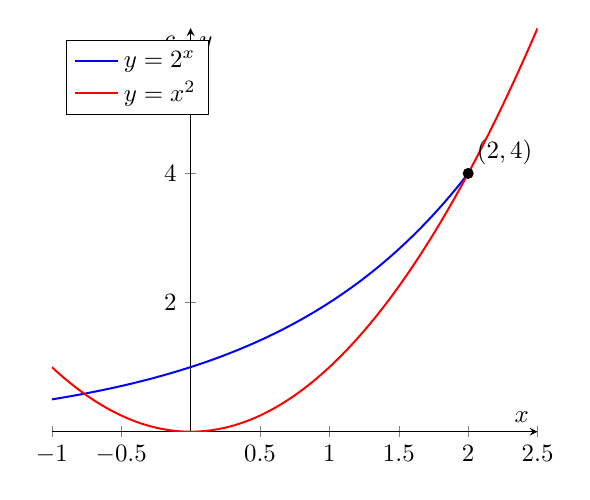
\begin{tikzpicture}[scale=0.9]
    \begin{axis}[
        axis lines = middle,
        xlabel = {$x$},
        ylabel = {$y$},
        legend pos = north west,
        legend cell align={left},
        samples = 100,
        domain = -1:2.5
    ]
    % Plot y = 2^x
    \addplot [
        domain = -1:2,
        smooth,
        thick,
        blue
    ] {2^x};
    \addlegendentry{$y=2^x$}

    % Plot y = x^2
    \addplot [
        domain = -1:2.5,
        smooth,
        thick,
        red
    ] {x^2};
    \addlegendentry{$y=x^2$}

    % Mark the point (2,4)
    \addplot[
        color = black,
        only marks,
        mark = *,
        mark size = 2pt
    ] coordinates {(2, 4)};
    \node[above right] at (axis cs:2, 4) {$(2, 4)$};
    
    \end{axis}
\end{tikzpicture}
\end{center}
\textit{Logarithmic form:}
$$x\log_2(2)=2\log_2(x) $$  
\textit{Integers Solutions:}
$$x=2, x=4$$
More possible solutions can be found here. \href{https://www.wolframalpha.com/input?i2d=true&i=Power%5B2%2Cx%5D%3DPower%5Bx%2C2%5D}{Lambert W function}
    \end{solution}
\end{enumerate}
2. Show that the line $y=-10x+20$ is tangent to the curve $y=x^4-4x^3-5x^2+26x-16$


\begin{solution}
Given the functions \( f(x) = x^4 - 4x^3 - 5x^2 + 26x - 16 \) and \( g(x) = -10x + 20 \), we find:

\[
f(x) - g(x) = x^4 - 4x^3 - 5x^2 + 36x - 36
\]

We factor \( f(x) - g(x) \) using synthetic division. Possible factors are \(\pm 1, 2, 3, 6, 12, 18, 36\).

First, we try \( x = 2 \):

\[
\polyhornerscheme[x=2]{x^4-4x^3-5x^2+36x-36}
\]

This gives us \((x - 2)(x^3 - 2x^2 - 9x + 18)\). We use synthetic division again on \( x^3 - 2x^2 - 9x + 18 \):

\[
\polyhornerscheme[x=2]{x^3-2x^2-9x+18}
\]

This results in:

\[
(x - 2)^2(x^2 - 9) = (x - 2)^2(x + 3)(x - 3)
\]

Finally, we find the tangent line \( y = -10x + 20 \) at \( x = 2 \):

\[
y = -10(2) + 20 = 0
\]

$\therefore$ The tangent points are \((2, 0)\).

\subsection*{Additional way using Calculus}
This question seems to be a calculus question too, so I decided to start with the curve:
    \begin{align*}
        &\text{First, find the first derivative of the curve:} \\
        y' &= 4x^3 - 12x^2 - 10x + 26 \\
        &\text{Then, set the derivative equal to the slope of the line:} \\
        &-10=4x^3 - 12x^2 - 10x + 26  \\
        &4x^3 - 12x^2 - 10x + 36 = 0 \\
        &\text{Greatest Common Factor is 2:}\\
        & 2(2x^3-6x^2-5x+18)=0 \\
\end{align*}
      I found possible numbers for this function is $(x-2)= 0$, which is 2 because I plugged and I got 0. Now, the next step comes the synthetic division, 
      $$\polyhornerscheme[x=2]{2x^3-6x^2-5x+18}$$

\begin{align*}
&\therefore 2(x-2)(2x^2-2x-9)=0\\
        &\text{Verify the point using the original function:} \\
        y &= x^4 - 4x^3 - 5x^2 + 26x - 16 \quad \text{at } x = 2 \\
        y &= (2)^4 - 4(2)^3 - 5(2)^2 + 26(2) - 16 \\
        y &= 16-32-20+52-16 = 0 \\
        &\text{Point of tangency: } (2, 0)
    \end{align*}
\end{solution}

3. Assume the cosine addition formula has been proven graphically.
\begin{enumerate}
    \item[a)] Prove the sine addition formula.
    \begin{solution}

    \begin{align*}
        \cos(a) &= \cos(a + b - b) \\
        &= \cos(a + b)\cos(b) + \sin(a + b)\sin(b) \quad \text{(Subtracting $b$ from both sides)} \\
        &= (\cos(a)\cos(b) - \sin(a)\sin(b))\cos(b) + \sin(a + b)\sin(b) \quad \text{(Cosine addition formula)}\\
        &= \sin(a + b)\sin(b) \quad \text{(Expanding)} \\
        &\text{Trig identity: $\cos(a)\cos(b) - \sin(a)\sin(b) = \sin(a + b)\sin(b)$.}\\
        &= \cos(a) - \cos(a)\cos^2(b) + \sin(a)\sin(b)\cos(b) \\
        &= (1 - \cos^2(b))\cos(a) + \sin(a)\sin(b)\cos(b) \quad \text{(Using identities)} \\
        &= \sin(b) \cdot (\cos(a)\sin(b) + \sin(a)\cos(b)) \quad \text{(Substituting $\sin^2(b) = 1 - \cos^2(b)$)} \\
    \end{align*}
    Hence, 
    \[
    \sin(a + b) = \cos(a)\sin(b) + \sin(a)\cos(b)
    \]

\textbf{Note:} If $\sin(b) = 0$, then $b = \pi \cdot n$, where $n$ is an integer. This implies $\cos(b) = (-1)^n$, as cosine alternates between $-1$ and $1$ at integer multiples of $\pi$, effectively alternating between ends of the circle. 

 $\therefore \quad \sin(a + b)$ simplifies to $(-1)^n \sin(a)$, which equals $\cos(b) \sin(a)$. Hence, the formula $\sin(a + b) = \cos(a)\sin(b) + \sin(a)\cos(b)$ still holds true.



    \end{solution}

    \item[b)] Derive the tangent addition formula.
    \begin{solution}
\begin{align*}
    \tan(a + b) &= \frac{\sin(a + b)}{\cos(a + b)} \quad \text{(Definition of tangent)} \\
    &= \frac{\sin a \cos b + \cos a \sin b}{\cos a \cos b - \sin a \sin b} \quad \text{(Expansion of sine and cosine)} \\
    &= \frac{\frac{\sin a \cos b + \cos a \sin b}{\cos a \cos b}}{\frac{\cos a \cos b - \sin a \sin b}{\cos a \cos b}} \quad \text{(Divide numerator and denominator by } \cos a \cos b) \\
    &= \frac{\frac{\sin a}{\cos a} + \frac{\sin b}{\cos b}}{1 - \frac{\sin a}{\cos a} \frac{\sin b}{\cos b}} \quad \text{(Rewrite in terms of tangent)} \\
    &= \frac{\tan a + \tan b}{1 - \tan a \tan b} \quad \therefore\text{(Definition of tangent)}
\end{align*}

    \end{solution}
\end{enumerate}

4. Stan invests \$1000 at 3\% compounded semi-annually and \$1500 at 1.8\% compounded annually. When will the two investments be equal?
\begin{solution}
    \begin{align*}
        A &= P\left(1 + \frac{r}{n}\right)^{nt} \\
        \text{For } \$1000 \text{ compounded semi-annually:} \\
        A_1 &= 1000\left(1 + \frac{0.03}{2}\right)^{2t} \\
        &= 1000\left(1 + 0.015\right)^{2t} \\
        \text{For } \$1500 \text{ compounded annually:} \\
        A_2 &= 1500\left(1 + 0.018\right)^t \\
        &= 1500(1.018)^t \\
        \text{Set } A_1 = A_2 \\
        1000(1.015)^{2t} &= 1500(1.018)^t \\
        \left(\frac{1.015^{2t}}{1.018^t}\right) &= \frac{1500}{1000} \\
        \left(\frac{(1.015)^2}{1.018}\right)^t &= 1.5 \\
        \left(\frac{1.030225}{1.018}\right)^t &= 1.5 \\
        (1.012085)^t &= 1.5 \\
        t &= \frac{\ln(1.5)}{\ln(1.012085)} \\
        \therefore t &\approx 34.56 \text{ years}
    \end{align*}
\end{solution}

5. Determine whether the following are equations or identities. If they are equations, solve them; otherwise, prove the identity. $x\in[0, 360^{\circ}]$
\begin{enumerate}
    \item[a)] $4\cos^2x = 3 - 2\sin^2x$
    \begin{solution}
        \begin{align*}
            4\cos^2x &= 3 - 2\sin^2x \\
            4\cos^2x + 2\sin^2x &= 3 \\
            4\cos^2x + 2(1 - \cos^2x) &= 3 \\
            4\cos^2x + 2 - 2\cos^2x &= 3 \\
            2\cos^2x &= 1 \\
            \cos^2x &= \frac{1}{2} \\
            \cos x &= \pm \frac{1}{\sqrt{2}} \\
            \therefore x &= 45^{\circ}, 135^{\circ}, 225^{\circ}, 315^{\circ}
        \end{align*}
    \end{solution}

    \item[b)] $\sin^4x + \cos^4x = \sin^2x (\csc^2x - 2\cos^2x)$
    \begin{solution}
        \begin{align*}
            LHS &\quad RHS\\
            \sin^4x + \cos^4x &= \sin^2x (\csc^2x - 2\cos^2x) \\
            &= \sin^2x \left(\frac{1}{\sin^2x} - 2\cos^2x\right) \\
            &= \sin^2x \left(\frac{1 - 2\cos^2x \sin^2x}{\sin^2x}\right) \\
            &= 1 - 2\cos^2x \sin^2x \\
            &= \sin^4x + \cos^4x \quad \text{(Identity)}\\
            \therefore RHS &= LHS
        \end{align*}
    \end{solution}

    \item[c)] $\frac{1 - \sin 2x}{\cos 2x} = \frac{\cos 2x}{1 + \sin 2x}$
    \begin{solution}
        \begin{align*}
            \frac{1 - \sin 2x}{\cos 2x} &= \frac{\cos 2x}{1 + \sin 2x} \\
            (1 - \sin 2x)(1 + \sin 2x) &= (\cos 2x)^2 \quad             \text{(Cross-multiply)} \\
            1 - \sin^2 2x &= \cos^2 2x \\
            \cos^2 2x &= \cos^2 2x \quad \text{(Identity)}
        \end{align*}
    \end{solution}

    \item[d)] $(\cot x)(\csc x)(\tan x)(\cos x) = \cos 2x + 2\sin^2x$
    \begin{solution}
        \begin{align*}
            (\cot x)(\csc x)(\tan x)(\cos x) &= \frac{\cos x}{\sin x} \cdot \frac{1}{\sin x} \cdot \frac{\sin x}{\cos x} \cdot \cos x \\
            &= \frac{\cos x \cdot 1 \cdot \sin x \cdot \cos x}{\sin x \cdot \sin x \cdot \cos x} \\
            &= \cos 2x + 2\sin^2x \quad \text{(Prove identity)}
        \end{align*}
    \end{solution}
\end{enumerate}

6. If $\sin x = \frac{12}{13}, \quad 0 < x < \frac{\pi}{2}$ and $\cos y = \frac{4}{5}, \quad -\frac{\pi}{2} < y < 0$, determine an exact value for $\sin[2(x-y)]$.
\begin{solution}
    \begin{align*}
        \sin x &= \frac{12}{13}, \quad \cos x = \frac{5}{13} \\
        \cos y &= \frac{4}{5}, \quad \sin y = -\frac{3}{5} \\
        \sin[2(x-y)] &= \sin 2x \cos 2y - \cos 2x \sin 2y \\
        &= 2\sin x \cos x \cdot 2\cos^2 y - 2\cos^2 x \cdot 2\sin^2 y \\
        &= 2 \left(\frac{12}{13} \cdot \frac{5}{13}\right) \cdot 2 \left(\frac{4}{5}\right)^2 - 2 \left(\frac{5}{13}\right)^2 \cdot 2 \left(\frac{3}{5}\right)^2 \\
        &= \frac{120}{169} \cdot \frac{32}{25} - \frac{50}{169} \cdot \frac{18}{25} \\
        &= \frac{3840}{4225} - \frac{900}{4225} \\
        &= \frac{2940}{4225}
    \end{align*}
\end{solution}

7. A mass on the end of a spring is pulled so that its distance from the rest position is initially 3cm. After being released, the mass oscillates while the spring contracts and expands. The motion of the mass is sinusoidal with a period of 3 seconds.
\begin{enumerate}
    \item[a)] Give the theoretical equation for the mass if it is distance from rest in terms of the time \( t \), in seconds, assuming no energy is lost with each cycle.
    \begin{solution}
        \begin{align*}
            y(t) &= 3 \cos\left(\frac{2\pi}{3} t\right)
        \end{align*}
    \end{solution}

    \item[b)] If the spring loses 5\% of its energy with each cycle, give the equation for this motion.
    \begin{solution}
        \begin{align*}
            y(t) &= 3 \left(0.95\right)^{\frac{t}{3}} \cos\left(\frac{2\pi}{3} t\right)
        \end{align*}
    \end{solution}
\end{enumerate}

8. The frets on a guitar are placed so that they make the correct vibrating string length for the note of music. We are interested in how the vibrating string length changes for each fret position. Below is the length from the bridge to each fret position.
\[
\begin{array}{|c|c|c|c|c|c|c|c|c|c|c|c|c|c|}
\hline
\text{Fret Number} & 0  & 1 & 2 & 3 & 4 & 5 & 6 & 7 & 8 & 9 & 10 & 11 & 12 \\
\hline
\text{Length (mm)} & 660 & 623 & 588 & 555 & 524 & 494 & 467 & 440 & 416 & 392 & 370 & 350 & 330 \\
\hline
\end{array}
\]
Using one of the methods from class determine the relationship between the fret number and the length 

\begin{solution}
The formula to calculate the distance from the bridge to the nth fret (\(D_n\)) is given by:
\[ D_n = D_0 \times \left(\frac{1}{2}\right)^{\frac{n}{12}} \]

Where:
\begin{itemize}
  \item \(D_0\) is the scale length (the distance from the bridge to the nut, which is the 0th fret).
  \item \(n\) is the fret number.
\end{itemize}

Using the given scale length of 660 mm, the lengths for the first few frets are calculated as follows:

\begin{align*}
D_2 &= 660 \times \left(\frac{1}{2}\right)^{\frac{2}{12}} \approx 588.00 \text{ mm} \\
D_5 &= 660 \times \left(\frac{1}{2}\right)^{\frac{5}{12}} \approx 494.00 \text{ mm} \\
D_9 &= 660 \times \left(\frac{1}{2}\right)^{\frac{9}{12}} \approx 416.00 \text{ mm} \\
D_{12} &= 660 \times \left(\frac{1}{2}\right)^{\frac{12}{12}} = 330.00 \text{ mm}
\end{align*}

In other words, the formula to calculate the distance from the bridge to the nth fret (\(D_n\)) is also can be log, which is:
\[ D_n = D_0 \times 2^{\frac{-n}{12}} \]

Where:
\begin{itemize}
  \item \(D_0\) is the scale length (the distance from the bridge to the nut, which is the 0th fret).
  \item \(n\) is the fret number.
\end{itemize}

This can also be expressed using logarithms as follows:
\[ D_n = D_0 \times 2^{\log_{2}\left(\frac{1}{2}\right)^{\frac{n}{12}}} \]

Same thing, using the given scale length of 660 mm, the lengths for the first few frets are calculated as follows:

\begin{align*}
D_2 &= 660 \times 2^{\log_{2}\left(\frac{1}{2}\right)^{\frac{2}{12}}} \approx 588.00 \text{ mm} \\
D_5 &= 660 \times 2^{\log_{2}\left(\frac{1}{2}\right)^{\frac{5}{12}}} \approx 494.00 \text{ mm} \\
D_9 &= 660 \times 2^{\log_{2}\left(\frac{1}{2}\right)^{\frac{9}{12}}} \approx 416.00 \text{ mm} \\
D_{12} &= 660 \times 2^{\log_{2}\left(\frac{1}{2}\right)^{\frac{12}{12}}} = 330.00 \text{ mm}
\end{align*}
\end{solution}

\subsubsection*{Graph - Relationship between Fret Number and Length}
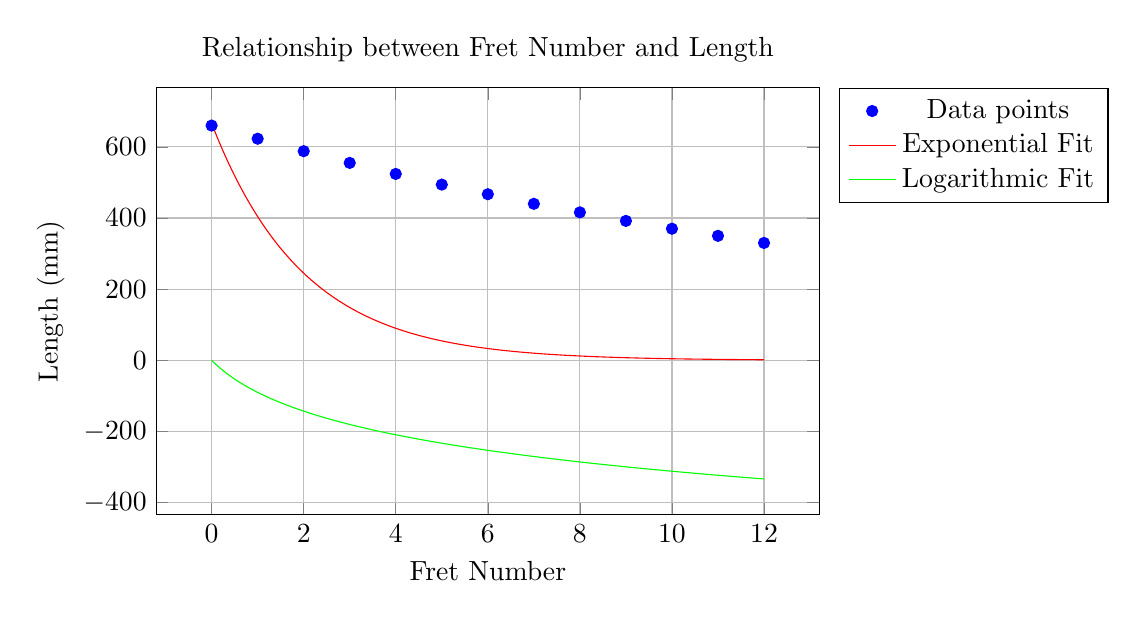
\begin{tikzpicture}
\begin{axis}[
    xlabel={Fret Number},
    ylabel={Length (mm)},
    title={Relationship between Fret Number and Length},
    grid=both,
    legend pos=outer north east,
    width=10cm,
    height=7cm
]
\addplot[only marks, mark=*, color=blue] coordinates {
    (0, 660)
    (1, 623)
    (2, 588)
    (3, 555)
    (4, 524)
    (5, 494)
    (6, 467)
    (7, 440)
    (8, 416)
    (9, 392)
    (10, 370)
    (11, 350)
    (12, 330)
};
\addlegendentry{Data points}

% Exponential fit
\addplot[domain=0:12, samples=100, color=red]{ 666 * exp(-0.5 * x)};
\addlegendentry{Exponential Fit}

% Logarithmic fit
\addplot[domain=0:12, samples=100, color=green]{-130 * ln(x + 1)};
\addlegendentry{Logarithmic Fit}
\end{axis}
\end{tikzpicture}

\vspace{2em}



9. I have \$100 dollars to invest, and I want to know how to allocate it between two possible entrepreneurs, Alpha and Beta, to maximize my total annual return.

\textit{Alpha: } If I give \( x \) dollars to Alpha, my annual return is \( A(x) = \frac{x(200-x)}{1000} \).

\textit{Beta: } If I give the remaining \( (100-x) \) dollars to Beta, my return is \( B(x) = r(100-x) \) dollars per year. That is, Beta simply pays me annual interest at rate \( r \).
\begin{enumerate}
    \item[a)] Take \( r = 12\% \) (that is, \( r = 0.12 \)). Using the given formula for \( A(x) \), find the allocation that maximizes the sum of my returns through Alpha and Beta. Illustrate your solution on a graph.



    
    \begin{solution}
        \begin{align*}
            \text{Total return: } R(x) &= A(x) + B(x) \\
            &= \frac{x(200-x)}{1000} + 0.12(100-x) \\
            &= \frac{200x - x^2}{1000} + 12 - 0.12x \\
            &= \frac{200x - x^2 + 12000 - 120x}{1000} \\
            &= \frac{-x^2 + 80x + 12000}{1000} \\
            &= -\frac{x^2}{1000} + \frac{80x}{1000} + 12 \\
            &= -\frac{x^2}{1000} + 0.08x + 12 \\
            \text{ My next idea comes take derivative:} \\
            R'(x) &= -\frac{2x}{1000} + 0.08 \\
            &= -0.002x + 0.08 \\
            \text{Set derivative to zero to find critical points:} \\
            0 &= -0.002x + 0.08 \\
            0.002x &= 0.08 \\
            x &= \frac{0.08}{0.002} \\
            x &= 40 \\
            \text{Check second derivative:} \\
            R''(x) &= -0.002 \\
            &< 0 \quad \text{(Maximum)}
        \end{align*}
       $\therefore$ The optimal allocation is \( x = 40 \) dollars to Alpha and \( 60 \) dollars to Beta.
    \end{solution}

    \item[b)] In case the optimal allocation is split, find a formula for the optimal allocation \( x \) in terms of the interest rate \( r \). What interest rates \( r \) would compel me to give everything to Beta?

    \begin{solution}
        \begin{align*}
            \text{Total return: } R(x) &= A(x) + B(x) \\
            &= \frac{x(200-x)}{1000} + r(100-x) \\
            &= \frac{200x - x^2}{1000} + 100r - rx \\
            &= \frac{-x^2 + (200 - 1000r)x + 100000r}{1000} \\
            \text{My next idea comes take derivative for this too:} \\
            R'(x) &= -\frac{2x}{1000} + \frac{200 - 1000r}{1000} \quad \text{(Divide)}\\
            &= -0.002x + 0.2 - r \\
            \text{Set derivative to zero to find critical points:} \\
            0 &= -0.002x + 0.2 - r \\
            0.002x &= 0.2 - r \\
            x &= \frac{0.2 - r}{0.002} \\
            x &= \frac{200(0.2 - r)}{0.002} \\
            \text{For } x \leq 0: \\
            0.2 - r \leq 0 \\
            r \geq 0.2 \\
            \text{For } x \geq 100: \\
            0.2 - r \geq 0.002 \cdot 100 \\
            r \leq 0.2
        \end{align*}
       $\therefore$ If \( r \geq 0.2 \), I should invest everything in Beta.
    \end{solution}
\end{enumerate}

10. After you eat something that contains sugar, the pH or acid level in your mouth changes. This can be modeled by the function $$ L(m) = \frac{-20.4m}{m^2+36} + 6.5, $$ where \textbf{L} is the \textbf{pH} level and \textbf{m} is the number of minutes that have elapsed since eating. Find the average rate of change from 1.5 minutes to 3 minutes, and find the instantaneous rate of change at 3 minutes.




\begin{solution}
    \begin{align*}
        \text{Average rate of change:} \\
        L(3) &= \frac{-20.4 \cdot 3}{3^2 + 36} + 6.5 \\
        &= \frac{-61.2}{45} + 6.5 \\
        &= -1.36 + 6.5 \\
        &= 5.14 \\
        L(1.5) &= \frac{-20.4 \cdot 1.5}{1.5^2 + 36} + 6.5 \\
        &= \frac{-30.6}{38.25} + 6.5 \\
        &= -0.8 + 6.5 \\
        &= 5.7 \\
       \therefore \text{Average rate of change:} \\
        &= \frac{L(3) - L(1.5)}{3 - 1.5} \\
        &= \frac{5.14 - 5.7}{1.5} \\
        &= \frac{-0.56}{1.5} \\
        &= -0.373 \\
        \text{Instantaneous rate of change(Literally calculus): } \\
        L'(m) &= \frac{d}{dm} \left( \frac{-20.4m}{m^2 + 36} + 6.5 \right) \quad \text{(Find derivative)}\\
        &= \frac{-20.4(m^2 + 36) - (-20.4m) \cdot 2m}{(m^2 + 36)^2} \quad \text{(Quotient rule)}\\
        &= \frac{-20.4m^2 - 734.4 + 40.8m^2}{(m^2 + 36)^2} \quad \text{(Simplify) } \\
        &= \frac{20.4m^2 - 734.4}{(m^2 + 36)^2} \\
        L'(3) &= \frac{20.4(3)^2 - 734.4}{(3^2 + 36)^2} \quad \text{(Plug 3)} \\
        &= \frac{183.6 - 734.4}{45^2} \\
        &= \frac{-550.8}{2025} \\
        &= -0.272
    \end{align*}
        $\therefore$ Instantaneous rate of change is (3, -0.272).
    
\end{solution}




\end{document}
